\documentclass[conference]{IEEEtran}


% *** CITATION PACKAGES ***
%
%\usepackage{cite}
% cite.sty was written by Donald Arseneau
% V1.6 and later of IEEEtran pre-defines the format of the cite.sty package
% \cite{} output to follow that of IEEE. Loading the cite package will
% result in citation numbers being automatically sorted and properly
% "compressed/ranged". e.g., [1], [9], [2], [7], [5], [6] without using
% cite.sty will become [1], [2], [5]--[7], [9] using cite.sty. cite.sty's
% \cite will automatically add leading space, if needed. Use cite.sty's
% noadjust option (cite.sty V3.8 and later) if you want to turn this off.
% cite.sty is already installed on most LaTeX systems. Be sure and use
% version 4.0 (2003-05-27) and later if using hyperref.sty. cite.sty does
% not currently provide for hyperlinked citations.
% The latest version can be obtained at:
% http://www.ctan.org/tex-archive/macros/latex/contrib/cite/
% The documentation is contained in the cite.sty file itself.


% *** GRAPHICS RELATED PACKAGES ***
%
\ifCLASSINFOpdf
  \usepackage[pdftex]{graphicx}
  % declare the path(s) where your graphic files are
  \graphicspath{{./imgs/}{../jpeg/}}
  % and their extensions so you won't have to specify these with
  % every instance of \includegraphics
  \DeclareGraphicsExtensions{.pdf,.jpg,.png}
\else
  % or other class option (dvipsone, dvipdf, if not using dvips). graphicx
  % will default to the driver specified in the system graphics.cfg if no
  % driver is specified.
  \usepackage[dvips]{graphicx}
  % declare the path(s) where your graphic files are
  \graphicspath{{../eps/}}
  % and their extensions so you won't have to specify these with
  % every instance of \includegraphics
  \DeclareGraphicsExtensions{.eps}
\fi
% graphicx was written by David Carlisle and Sebastian Rahtz. It is
% required if you want graphics, photos, etc. graphicx.sty is already
% installed on most LaTeX systems. The latest version and documentation can
% be obtained at: 
% http://www.ctan.org/tex-archive/macros/latex/required/graphics/
% Another good source of documentation is "Using Imported Graphics in
% LaTeX2e" by Keith Reckdahl which can be found as epslatex.ps or
% epslatex.pdf at: http://www.ctan.org/tex-archive/info/
%
% latex, and pdflatex in dvi mode, support graphics in encapsulated
% postscript (.eps) format. pdflatex in pdf mode supports graphics
% in .pdf, .jpeg, .png and .mps (metapost) formats. Users should ensure
% that all non-photo figures use a vector format (.eps, .pdf, .mps) and
% not a bitmapped formats (.jpeg, .png). IEEE frowns on bitmapped formats
% which can result in "jaggedy"/blurry rendering of lines and letters as
% well as large increases in file sizes.
%
% You can find documentation about the pdfTeX application at:
% http://www.tug.org/applications/pdftex

% correct bad hyphenation here
\hyphenation{op-tical net-works semi-conduc-tor}
\usepackage{rotating}
\usepackage{slashbox}
\usepackage{amsmath}
\usepackage{multirow}

\begin{document}
%
% paper title
% can use linebreaks \\ within to get better formatting as desired
\title{Using Developer Preferences to Improve Code Smell Detection}


% author names and affiliations
% use a multiple column layout for up to three different
% affiliations
\author{
\IEEEauthorblockN{Mario Hozano}
\IEEEauthorblockA{Federal University of Campina Grande\\
Department of Computing Systems\\
Campina Grande, Paraiba, Brazil\\
Email: mario@copin.ufcg.edu.br}
\and
\IEEEauthorblockN{Henrique Ferreira}
\IEEEauthorblockA{Federal University of Alagoas\\
Campus Arapiraca\\
Arapiraca, Alagoas, Brazil}
\and
\IEEEauthorblockN{Baldoino Fonseca\\ and Evandro Costa}
\IEEEauthorblockA{Federal University of Alagoas\\
Computing Institute\\
Maceio, Alagoas, Brazil}
Email: \{baldoino,evandro\}@ic.ufal.br}

% make the title area
\maketitle


\begin{abstract}

Identify the parts of code that needs a refactoring is a key activity of the refactoring process. After all, identifying refactoring opportunities concentrates big part of the effort spent in a refactoring task. Although efforts to develop automatic techniques to detect design problems were initiated many years ago, the identification task still present as a challenge looking for results with more relevance for developers. Tools that promise to make this activity do not cover a large variety of smells and, when used, the suggested smells reveals low agreement among them. It seems that tools are prepared to detect smells according to the understanding of the developers that created them. However, the meaning of bad smells can be different to the developers of the analyzed project. Against such scenario, we made a study to verify this issues and proposes a platform that integrates several approaches to 
identify bad smells in object oriented software projects. Such platform will allow use different techniques to detect refactoring opportunities over the same target project. In addition, the platform uses developer observations to infer the developer understanding about the smell and make use of this information to improve the identification process.

\end{abstract}
% IEEEtran.cls defaults to using nonbold math in the Abstract.
% This preserves the distinction between vectors and scalars. However,
% if the conference you are submitting to favors bold math in the abstract,
% then you can use LaTeX's standard command \boldmath at the very start
% of the abstract to achieve this. Many IEEE journals/conferences frown on
% math in the abstract anyway.

% no keywords




% For peer review papers, you can put extra information on the cover
% page as needed:
% \ifCLASSOPTIONpeerreview
% \begin{center} \bfseries EDICS Category: 3-BBND \end{center}
% \fi
%
% For peerreview papers, this IEEEtran command inserts a page break and
% creates the second title. It will be ignored for other modes.
\IEEEpeerreviewmaketitle



\section{Introduction}
\label{sec:introduction}

The real-world environment demands constant changes in business rules, which 
implies in new software requirements. By adding, removing and adapting 
features, the actual software systems needs a well-defined structure to allow 
its evolution easier, allowing to reduce software maintenance costs. In this 
sense, the refactoring process has been investigated as an effective activity
to increase software quality by achieving high cohesion, low coupling and code 
flexibility in programs\cite{Kataoka2002b,Ouni2012f}.

Opdyke, defines refactoring as a process of changing a software 
system in such a way that it does not alter the external behavior of the code, 
yet improves its internal structure~\cite{Opdyke:1992}. Such process begins with
the identification of the part of code that needs an improvement, and
follows with a software restructuring that refines the program and preserves its 
external behavior.

Identify the parts of code that needs a refactoring is a key activity of this 
process. Normally, identifying refactoring opportunities concentrates big part 
of the effort spent in a refactoring task. In addition, the use of 
non-automatic techniques to perform this task, increases the maintenance costs 
because the it is time expensive, unrepeatable and 
non-scalable problem~\cite{Marinescu2001c,Schumacher2010d}. The several situations where the 
code can be restructured and the high occurrences of them in object-oriented 
software, encourages researchers to investigate automatic techniques to detect 
refactoring opportunities.

Although efforts to develop automatic techniques to detect design problems were 
initiated many years ago~\cite{Ciupke:1999}, several works aims to create and 
adapt techniques to improve its efficiency, covering and 
applicability~\cite{Kessentini2011q, Fontana2012c, Khomh2009c, Ouni2012f}.

Mens and Tourwe~\cite{Mens2004b} describes techniques to 
detect design flaws in many approaches. The first, identify parts of the 
code that should be refactored through program invariant 
detection~\cite{KataokaEGN01}. Invariants may be parameters of a method that is 
always constant when invoked by a test suite or in a production use. In this 
way, this technique presents limitation by the guarantees that tests will cover 
all possible runs of a program and, consequently, the method's execution. 
Moreover, several design flaws are not associated with invariant behavior, but 
with other factors (e.g. readability, dependency, reuse, performance 
etc.) with no relation with constant value setting~\cite{kim2012field}.

Against the program invariant technique, the most widespread approach have considered 
software metrics (\cite{chidamber1994metrics,Gueheneuc:2004}) to identify parts 
of code that require refactoring, known as \textit{bad 
smells}~\cite{FowlerMartin2002}. In~\cite{FowlerMartin2002} Fowler and Beck 
describes a catalog that exemplifies and suggests changes to remove more than 20 
bad smells. This catalog is uses as basis of several techniques and tools.

Despite the Fowler's catalog describe details of how bad smells are presented 
in code, determine how to use software metrics to find these have becoming a 
hard task, mainly by two issues. The first problem is to associate 
specific smell characteristics with appropriate software metrics. In some cases 
such task can be simple than others. For example the \textit{Long Parameter 
List} smell is defined as a method with a huge quantity of parameters in his 
signature, difficulty to understand and evolve the software. In this 
case,~\cite{Gueheneuc:2004} presents a framework that retrieves the number of 
parameters of a given method through a metric named \texttt{NOParam}. In other 
hand, the bad smell \textit{Blob} (or \textit{God Class}) corresponds to a 
large controller class that depends on surrounding data classes. Such class 
monopolises most of the processing and decisions done by a 
system~\cite{Moha2010c}. According to its characteristics, metrics related to 
cohesion (e.g. LCOM, CAM)\footnote{LCOM - Lack of cohesion in methods, CAM -  
Cohesion Among Methods of Class~\cite{chidamber1994metrics}}, class/methods 
size (e.g. WMC, LOC)\footnote{WMC - Weighted methods per class, LOC - Lines of 
Code~\cite{chidamber1994metrics}} and accessing/coupling (e.g. CBO, 
DAM)\footnote{CBO - Coupling between object classes, DAM: Data Access 
Metric~\cite{chidamber1994metrics}} have been used in several researches trying 
to define rules to identify \textit{Blob} classes 
(\cite{Marinescu2001c,Moha2010c,Ouni2012f}).

The second problem is focused in the refinement of those techniques 
to detect bad smells efficiently in real systems. Even in the simple detection 
of \textit{Long Parameter List} described above, the thresholds to consider an specific 
smell can be different by developers. Once the bad smell's meaning is informal, 
the application of a specific value to \texttt{NOParam} metric can vary 
depending of the developer's experience, understanding and the software 
domain. The ambiguity of the smell definitions, the different 
detection techniques and the different threshold values provide, justify 
different results when a system is analyzed by different tools as presented 
in~\cite{Fontana2012c}. This subjective nature have motivated researchers to 
investigate appropriated thresholds~\cite{Paloma:2014,Kessentini2010c}, 
determine new approaches to detect smells~\cite{Palomba2013d,Ouni2013h} and use 
intelligent techniques~\cite{Khomh2009c,Ouni2012f}.

These different techniques, thresholds and understanding about smell 
detection context, reflect a complex scenario to do this activity in software 
development life-cycle. Actually, several tools help developers to identify bad 
smells using different approaches, each them aims to specific smells, and 
produces different results. Fontana et al.~\cite{Fontana2012c} 
present an experiment where four different tools do not meaningfully agree in 
their answers to detect specific smells in a medium-size software project. Such 
work still presents that needs at least 6 tools to try identifying only 6
bad smell types.

Considering the relevance of the smell identification task in a software 
development, and the low efficiency, covering and 
applicability in the available tools, becomes important define a platform that 
combines identification techniques to improve the results of this task, helping 
developers. This platform will allow increase accuracy and perform this 
activity covering a major range of bad smells type.

In this paper, we proposes a platform that integrates several approaches to 
identify bad smells in object oriented software projects. Such platform will 
allow use different techniques to detect refactoring opportunities over the 
same target project. Thus, the results of these techniques can be used to 
increment accuracy and covering, helping developers in this importante task. 
Section~\ref{sec:motivation} details the smell identification by using an 
illustrative example. Section~\ref{sec:approach} describes our proposed 
approach. In~Section~\ref{sec:tool} we present how the proposed approach can be 
defined as a real tool to help developers and Section~\ref{sec:study} shows how 
it can be applied in a controlled experiment. Results about this study 
is presented in Section~\ref{sec:results}. Related works are presented in 
Section~\ref{sec:related} and, finally, Section~\ref{sec:conclusion} concludes 
this work.



%[comment] Pessoal a introduction pode seguir o roteiro abaixo
%Contexto
%Problema
%Por que é interessante?
%Relevante?
%Hipótese
%Um pouco da solução
%Como resolver o problema?
%Por que é original?
%Por que dá pra resolver?
%Por que eu consigo?
%Resultados


\section{Motivating Example}
\label{sec:motivation}

To illustrate the actual scenario in bad smell identification field, we describe a real example to show the difficulties dealing with identification of refactoring opportunities using appropriate tools. In such example we concentrates the bad smell identification into four well known bad smells following described:

\begin{itemize}
 \item \textbf{God Class} (also called Blob) refers to class that tends to centralize the intelligence of the system. A God Class performs too much work on its own, delegating only minor details to a set of trivial classes, and using the data from other classes~\cite{Lanza:2005}. 
 
 \item \textbf{Long Parameter List} is a parameter list that is too long and thus difficult to understand. It can be hard to work with because both caller and callee have to remember which values were there. They also encourage duplicate code because the called object can't take advantage of any other methods on the whole object to calculate intermediate values~\cite{FowlerMartin2002}.
 
 \item \textbf{Long Method} is a method that is too long, so it is difficult to understand, change, or extend. The Long Method tend to centralize the functionality of a class, in the same way as a God Class centralizes the functionality of an entire subsystem, or sometimes even a whole system~\cite{Fontana2012c}.
 
 \item \textbf{Feature Envy} means that a method is more interested in other class(es) than the one where it is currently located. This method is in the wrong place since it is more tightly coupled to the other class than to the one where it is currently located~\cite{Fontana2012c}.
\end{itemize}

To detect these smells we used four tools widely used to identify refactoring opportunities. Such tools are briefly described below, as well as its version used in this example:

\begin{itemize}
 \item \textbf{PMD}~\cite{PMD} is a source code analyzer. It finds common programming flaws like unused variables, empty catch blocks, unnecessary object creation, and so forth. Version used: 5.1.1.
 \item \textbf{CheckStyle}~\cite{Checkstyle} is a development tool to help programmers write Java code that adheres to a coding standard. It automates the process of checking Java code to spare humans of this boring (but important) task. This makes it ideal for projects that want to enforce a coding standard. Version used: 5.7.
 \item \textbf{JDeodorant}~\cite{JDeodorant} is an Eclipse plug-in that identifies design problems in software, known as bad smells, and resolves them by applying appropriate refactorings. Version used: 5.0.
 \item \textbf{inFusion}~\cite{inFusion} aggregates metrics, visualizations and other static analysis techniques, to produce intuitive insights, semantics-rich interpretations and matching refactoring recommendations, which identify and address inadequate underlying design decisions. Version used: 1.8.5.
\end{itemize}

We submit these tools to detect refactoring opportunities in a medium-size open source project known as GanttProject, a cross-platform desktop tool for project scheduling and management~\cite{GanttProject}. The version 2.0.10, used in this example, has ??? Java classes distributed in ???? lines of code. The results got in this motivating example as described in Table~\ref{tab:motivation}.

\begin{table}[h]
\centering
\caption{Identification Tools Comparison}
\label{tab:motivation}
\begin{tabular}{|c||c|c|c|c|c|c|}
\hline
{Analyzed Smells}& \multicolumn{1}{l|}{\begin{sideways}inFusion\end{sideways}} & \multicolumn{1}{l|}{\begin{sideways}JDeodorant~~\end{sideways}} & \multicolumn{1}{l|}{\begin{sideways}Checkstyle\end{sideways}} & \multicolumn{1}{l|}{\begin{sideways}PMD\end{sideways}} & \multicolumn{1}{l|}{ \# Smells} & \multicolumn{1}{l|}{ \% Agreement} \\ \hline \hline
God Class	& 17 & 43  & \begin{math}\times\end{math} &  \begin{math}\times\end{math} & 50 & 20.0\%                \\ \hline
Long Parameter List & \begin{math}\times\end{math} & \begin{math}\times\end{math}   & 1 & 0   & 1 & 0.0\%                  \\ \hline
Long Method     & \begin{math}\times\end{math} & 108   & 13  	& 14  &   127 &   1.5\%    \\ \hline
Feature Envy     & 12 & 49 & \begin{math}\times\end{math}  & \begin{math}\times\end{math}  &   61 &   0.0\%  \\
\hline
\end{tabular}
\end{table}

Analyzing the results got in smell identification using the tools and smells listed above, we can verify some difficulties to perform this task in a real scenario. For example, to verify only four bad smells, well known in literature, was needed at least two identification tools. No one listed tool allow detect all smell analyzed in our example. In such case, Checkstyle and PMD do not provide mechanisms to identify God Class and Feature Envy smells, inFusion does not provide support to identify Long Parameter List and Long Method, while JDeodorant, does not detect Long Parameter List. Considering the importance to verify a great variety of bad smells, trying to improve the software quality and reducing maintenance costs, it is needed to use several tools to get a good coverage in smell identification. For example, Fontana et al.~\cite{Fontana2012c} present an experiment where six different tools (including all used in our example) is needed to try identifying only 6 bad smell types. The form of how each smell is presented in source code, can justify why some techniques (or tools) does not work identifying a great variety of smells. Efforts have been made to classify smells in categories according with its nature (e.g measurable, lexical, structural, intra-class, inter-class)~\cite{Wake:2003,Mantyla:2003}.

Beyond the coverage problem, another issue is showed analyzing the results of each tool. Analyzing a specific smell using more than one tool is it possible to realize a low agreement joining its results. Indeed, Table~\ref{tab:motivation} present the better agreement was not more than 20\% identifying 10 from 50 God Classes using inFusion and JDeodorant tools. The results over the others smells shows that the quantity of identified smell is not related with better or worse agreement. The same tools has detected 61 Feature Envy smells with no identification in common. In Long Parameter List results we have no agreement, too. Nevertheless, in this case, Checkstyle and PMD, has detected only 1 unique smell of this kind. Finally, the Long Method was the unique smell supported by three tools: JDeodorant, Checkstyle and PMD. In this case we had the major detection, with 127 smells, but the agreement among tools continues very low with only 2 detection cases (1.5\%). 

The low agreement detailed above reflects a great challenge to smell identification field. In this scenario, subjective issues must be investigated, and two factor contributes with those worse results. 

Firstly, the different understanding about the smell, implies differences in strategies to detect them. For example, several tools (including inFusion) adopts the strategy proposed by Lanza and Marinescu~\cite{Lanza:2005} to detect God Classes through the computation of three metrics (WMC\footnote{Weighted Method Count: the sum of the statistical complexity of all methods in a class.}, TCC\footnote{Tight Class Cohesion: the relative number of methods directly connected via accesses of attributes.}, and ATFD\footnote{Access to Foreign Data: the number of external classes from which a given class accesses attributes, directly or via accessor methods.}). In other hand, JDeodorant adopts another strategy that computes a God Class as a class that can be decomposed in other classes~\cite{Fontana2012c}, using other metrics. 

Second, even in cases where the tools agree with the strategy to detect a specific smell using the same metrics to detect them, the values used as thresholds of these metrics implies in different results on detection process. In case of Long Parameter List, Checkstyle and PMD computes the number of parameters of each method, defining a metric known as NOPARAM. However, while Checkstyle considers smells all methods with \texttt{NOPARAM \textgreater~7}, PMD uses this thresholds value adjusted to 10. The same problem occurs detecting Long Method, where both tools uses the metric MLOC\footnote{Number of lines of code in method}. While Checkstyle considers Long Method all methods with \texttt{MLOC \textgreater~150} and PMD considers \texttt{MLOC \textgreater~100}. 

In such scenario we can found tools to detect bad smells with generic rules, trying to satisfy a great demand of projects but decreasing its precision, suggesting a lot of false positives to developer. Or, in other case, tools using specific rules with high precision, but that not able to be used with a great variety of projects and do not detect all smells in the analyzed project.

These two issues help to explain why actual tools presents different results when submitted to analyze software. The tools are prepared to detect smells according to the understanding of the developers that developed them. But the meaning of bad smells can be different to the developers of the analyzed project. The actual tools must consider the literature about the smell identification, including metrics that reflects inadequate or bad practice in a software design. Nevertheless, they can not forget that the understanding of bad smells is a subjective field, that depends of the meaning considered by the developers that will be assisted, and the context where the analyzed software is defined. To contribute with this challenge in refactoring field, we propose a platform to improve the results in bad smell identification by assisting actual techniques with data about the software context and observations made by the assisted developers. In addition, to avoid the re-computation of metrics used by two or more techniques, our platform provides a component to share metrics about the analyzed software according from real-time observations in source code. The Section~\ref{sec:approach} describes such platform.

\section{Smell Platform}
\label{sec:approach}

The Smell Platform was built to integrate different techniques to identify refactoring opportunities and help this process with important data about the software to be analyzed. The techniques are disposed as sniffers that identify bad smells in software projects. 

Once the most widespread techniques have considered 
software metrics to identify refactoring opportunities~\cite{marinescu2004detection,salehie2006metric}, the Smell Platform supports a mechanism to calculate and share metrics that can be used by the sniffers. 

Although some studies report successes smell identification with software metrics, the use of them must be done together with setting definitions about the software domain, developer/team preferences and other adjusts to get good and relevant results about this process. Thus, the use of metrics are supported with data about developer preferences, inferred from developer analysis by approve or reject the suggested smells. 

\begin{figure}[!t]
\label{fig:flow}
\centering
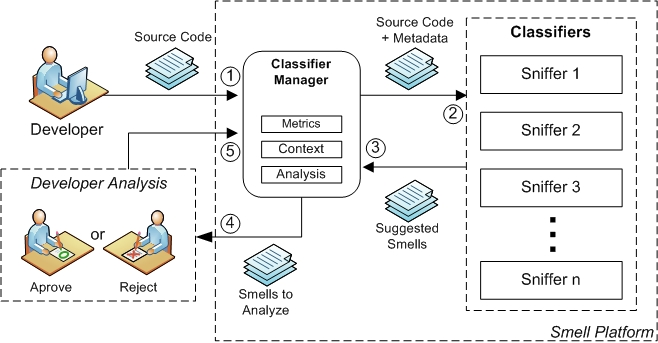
\includegraphics[natwidth=658px, natheight=343px, width=230px]{imgs/flow.jpg}
\caption{Smell Platform Execution Flow}
\end{figure}

Figure~\ref{fig:flow} illustrates the Smell Platform execution flow. The process is started in step 1, where the developer submits the source code of the project to be analyzed by the platform. The Sniffer Manager processes the metrics related to the software and stores them using the Metrics component. These metrics will be shared with all Sniffers, avoiding re-processing to calculate them individually. Besides metrics, the Sniffer Manager bundles context information to help sniffers to consider the subjective issues about the target software and, consequently, improving the results in smell identification. The context information are managed by the Context component through user setting (before this execution) and inferences over the target project. Once that metrics and context data are processed, these data passed by the Sniffer Manager to all Sniffers in the platform (step 2). The sniffer is responsible to encapsulate a technique to identify bad smells using the source code of the target project and the shared information about context and metrics. In this scenario it is possible to use different intelligent techniques already used to perform this task isolatedly, as Bayesian Networks~\cite{Khomh2009c}, Genetic Programming~\cite{Ouni2012f}, Association Rule~\cite{Using2013c}. The results obtained from each sniffer are passed to Sniffer Manager (step 3), where they are grouped and filtered before show results with the suggested smells to developer (step 4). The results must present the bad smell name, the specific part of code where this smell is placed and an explanation showing why it was considered a bad smell. According to such information, the developer can analyze the results received by the Sniffer manager, and approve or reject, individually, each presented suggestion. All analysis are stored by the Analysis Component in the Smell Platform (step 5), to help the execution of the smell identification in further iterations. It can be used to infer context information, like developer preferences, and help sniffers to increase its accuracy on smell identification using them.

Considering the execution flow presented above, the Smell Platform was developed using a simple architecture illustrated in Figure~\ref{fig:arch} and detailed in the following sections.

\begin{figure}[!h]
\label{fig:arch}
\centering
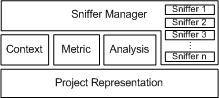
\includegraphics[natwidth=219px, natheight=98px, 
width=170px]{imgs/arquitetura.jpg}
\caption{Smell Platform Architecture}
\end{figure}

\subsection{Project Representation}

The Project Representation layer represents a basis to Smell Platform. In this layer are implemented mechanisms to parse the source code about the project that will be analyzed, and represent it in a structure used by sniffers. In refactoring context, an commom structure used by tools to help smell identification is an Abstract Syntax Tree (AST) representing the source code~\cite{Koschke2006,Mens02formalisingbehaviour,Baxter:1998}. An AST can be defined as a tree of nodes representing constants or variables, and operators or statements. However, the platform allows use others formalisms to represent the project, by extending its capabilities.

\subsection{Metric}

As mentioned in Section~\ref{sec:introduction}, the most widespread techniques have considered 
software metrics to identify refactoring opportunities~\cite{marinescu2004detection,salehie2006metric}. In this scenario, the Metric component is built to help sniffers calculating and supplying metrics to them. In addition to traditional software metrics, such component provides an extension point that allows developers to enable new metrics in the smell platform, as used in the recent researches~\cite{Padilha:2013,Palomba2013d}.

\subsection{Analysis}

According to the execution flow, illustrated in Figure~\ref{fig:flow}, the refactoring opportunities observed by the Sniffers are showed to developer (step 4). At this moment, the developer can make a subjective analysis about the results of the sniffers using different techniques. All human analysis are stored by the Analysis Manager and shared with sniffers to allow intelligent mechanisms to improve its results through the approved or rejected analysis. 

\subsection{Context}

The Context component manages information about the software domain, developer preferences, experience etc. It support sniffers providing initial information about the use of metrics setting manually or inferred by the the source code and developer analysis~\cite{Paloma:2014}. 

\subsection{Sniffer Manager}

The main layer of the Smell Platform architecture is the Sniffer Manager. Such layer concentrates all work focused in the smell identification with techniques encapsulated in Sniffer Components. Each Sniffer can be implemented to detect smells internally or adapt that task to use an external existing component, technique or tool. In this scenario all sniffers can use the metrics, analysis and context information described above and/or process other data individually in its work. The results produced by the sniffers must present the bad smell name, the specific part of code where this smell is placed and an explanation showing why it was considered a bad smell.

\section{Study Settings}
\label{sec:study}

Continuing our efforts, we conduct a study focused to validate our approach against the problems described in Section~\ref{sec:motivation}. Our study aims at analyze the efficiency in bad smell detection using information supplied by the developers that are exploring the project that is been analyzed, in the context of code refactoring in object-oriented software. In this case, the efficiency should be considered from the viewpoint of developers themselves, who will be assisted by tools for this purpose. In this case, we perform a comparative analysis between smells suggested by the existent tools and using our approach, supported with information about the developer preferences. The Section~\ref{sec:questions} discusses the research questions of this study. Section~\ref{sec:systems} present the bad smells and the projects that will be analyzed. Section~\ref{sec:subjects} describes the subjects that took part in this study. Section~\ref{sec:instrumentation} describes the instruments used in the study and, finally, Section~\ref{sec:operation} explains how the study was done.

\subsection{Research Questions}
\label{sec:questions}

The goal of this study is to find out whether information about the developer's understanding about the design flaws and the software domain, can improve the smell detection results. Therefore, the main research question we aim to answer can be defined as follows:

\begin{flushleft}
Q1: Can developer preferences help in bad smell detection?
\end{flushleft}

While this study is conducted to answer the main research question, other specific questions can be derived in our investigation:

\begin{flushleft}
% Q2: Does the proposed approach is effective in bad smell detection?

Q2: Can developer preferences help to detect smells more precisely?

Q3: Can developer preferences be inferred from analysis over suggested smells?

% Q4: How accurate do our approach perform in comparison with traditional ones in detection process ?

\end{flushleft}

\subsection{Target Systems, Tools and Smells}
\label{sec:systems}

Our study involved the four bad smells described in Section~\ref{sec:motivation}: God Class, Long Parameter List, Long Method and Feature Envy. These smells were investigated by the tools inFusion, JDeodorant, Checkstyle, and PMD, according to the support offered by each system. The investigation happened in two open-source systems: GanttProject~\cite{GanttProject}, previously introduced in Section~\ref{sec:motivation} and Xerces, a library for parsing, validating and manipulating XML documents~\cite{Xerces}. These systems were selected because we have access to the code and they are projects already used in other studies in bad smell identification~\cite{Moha2010c, Ouni2012f, Palomba2013d}. Table~\ref{tab:study} detail the projects characteristics.

\begin{table}[ht]
\centering
\caption{Projects analyzed in Study}
\label{tab:study}
\begin{tabular}{lccc}
\hline
Name         & \multicolumn{1}{l}{Version} & \multicolumn{1}{l}{Lines of Code} & \multicolumn{1}{l}{Classes} \\ \hline
GanttProject & 2.10.2                       & 45.070                             & X                            \\ 
Xerces       & 2.11.0                       & X                                  & X                            \\ \hline
\end{tabular}
\end{table}


\subsection{Subject Selection}
\label{sec:subjects}

The study was conducted in an academic environment with 4 students on graduate level and 2 software engineers with at least 3 years experience. Although these individuals have not collaborating with the development of the analyzed projects, they have experience in identifying bad smells.

\subsection{Instrumentation}
\label{sec:instrumentation}

The background and experience of the individuals was collected through a survey delivered before the analyzing process begins. 

During the analyzing phase a list of suggested smells were delivered to each participant. Such list presents a subset of the smells suggested by the tools during the GanttProject's analysis (Table~\ref{tab:motivation}). To prevent the study become tiring, each participant receive a list with up to 20 random smells of each kind. 


\subsection{Operation}
\label{sec:operation}

The study was started with a 30-minute training session to allow subjects to familiarize themselves with the environment and the target code smells. After this session, a work station with Eclipse IDE~\cite{Eclipse} installed and the source code of GanttProject opened as an Eclipse Project, was dedicated to each subject. At this moment, each subject received a document containing a list with all smells identified by the four tools in GanttProject. The document also described steps and guidelines that subjects should follow and information they should register. The individuals were instructed to analyze the suggested smells in document and inform whether he approves or rejects the suggestion.

After two hours, all documents was collected containing all analysis made by subjects over the smells suggested in GanttProject, verified by tools before. The observations about approvals and rejections were analyzed and processed to infer information about the developer preferences, that could improve a future smell identification process. 

Two days after, all subjects were invited to perform another similar analysis in other round. However, in this turn they were presented to the Xerces project and the list of suggested smells were filtered according to its preferences inferred by the analysis informed in the first round. Each subject receive a different list fitted according to its previously validation. Again, the subjects were instructed to approve or reject all smells indicated in its list analyzing the Xerces code. At the end, all analysis were collected and its results were processed to be compared with the previously analysis. Both in the first round as the second, subjects were not informed that lists were produced from results of tools for checking bad smells.


% Research Questions
% Subject Selection*
% Instrumentation
% Operation*
% 


\section{Results and Discussion}
\label{sec:results}

After the first round of our study, described in Section~\ref{sec:study}, we collect all analysis made by the participants and evaluate the accuracy of the approved smells against the smell suggested by tools. In this case, we calculate the precision metric as follows:

\begin{equation*}
 precision = \frac{number~of~approved~smells}{number~of~suggested~smells}
\end{equation*}

Table~\ref{tab:turn1} details the results gathered after the first round where the 6 subjects evaluate whether the suggested smells are or not bad smells. The table rows details the results obtained from each subject against the four smells described in columns. Each cell present the number of smells approved followed by the smells analyzed, while the percentage of the precision metric is described in parenthesis.

\begin{table}[h]
\centering
\caption{Smells Analyzed by Humans over GanttProject}
\label{tab:turn1}
\begin{tabular}{crrrrr}
\hline
Subject & \multicolumn{1}{r}{Long Param. List}       & \multicolumn{1}{r}{God Class}          & \multicolumn{1}{r}{Feature Envy}           & \multicolumn{1}{r}{Long Method}  \\ \hline
1        & \multicolumn{1}{r}{0/1 (0.00)} & \multicolumn{1}{r}{6/19 (31.58)} & \multicolumn{1}{r}{15/20 (75.00)} & 7/20 (35.00)                \\ 
2        & 0/1 (0.00)                      & 5/20 (25.00)                      & 7/20 (35.00)                       & 4/17 (23.53)             \\ 
3        & 1/1 (100.00)                    & 4/20 (20.00)                      & 7/19 (36.84)                       & 9/20 (45.00)             \\ 
4        & 1/1 (100.00)                    & 6/20 (30.00)                      & 2/20 (10.00)                       & 5/20 (25.00)             \\ 
5        & 1/1 (100.00)                    & 9/19 (47.37)                      & 8/20 (40.00)                       & 3/20 (15.00)             \\ 
6        & 1/1 (100.00)                    & 13/19 (68.42)                     & 18/20 (90.00)                      & 7/20 (35.00)             \\ \hline
\end{tabular}
\end{table}

The smells analyzed in the first round reveals low precision in all smells, except in Long Parameter List. Only an unique smell was suggested by the Checkstyle tool as Long Parameter List in a constructor with 9 parameters. Nevertheless, two subjects (1 and 2) disagree that this suggestion is a bad smell. Considering the other three smells, the precision was measured with values below 50 percent in several cases. 

At this point, we recall the research questions which motivated him to continue discussing about the study results in the following sections.

\subsection{Can developer preferences be inferred from analysis over suggested smells?}

Considering the values described in Table~\ref{tab:turn1}, the Smell Platform has used two strategies to infer developer's preferences from analysis data, and improve the precision in the next study round. The first, has defined specific thresholds to detect Long Methods and Long Parameter List smells, using respectively the lowest values of MLOC and NOPARAM from the approved smells in the first round from each subject. In case where no smell was approved (like Long Parameter List analysis from subjects 1 and 2), a most restrictive threshold was defined with NOPARAM \textgreater~10. The second strategy was defined to infer preferences to detect God Class and Feature Envy smells. Once only JDeodorant and inFusion tools support the identification of these smells, and these do not provide mechanisms to adjust the smell identification by using developer preferences, the smell platform inferred the most appropriated tool to each subject. The choose was defined by the precision analyzed into the smells suggested from each tool individually. Table~\ref{tab:strategies} illustrates the preferences inferred by Smell Platform from analysis in the first round of the study.

\begin{table}[h]
\centering
\caption{Preferences inferred by Smell Platform}
\label{tab:strategies}
\begin{tabular}{cccccc}
\hline
Subject & \multicolumn{1}{r}{Long Param. List}       & \multicolumn{1}{r}{God Class}          & \multicolumn{1}{r}{Feature Envy}           & \multicolumn{1}{r}{Long Method}  \\ \hline
1        & \multicolumn{1}{c}{NOPARAM \textgreater~10} & \multicolumn{1}{c}{inFusion} & \multicolumn{1}{c}{inFusion} & LOC $\geq$ 49 \\ 
2        & NOPARAM \textgreater~10         & inFusion                      & inFusion                       & LOC $\geq$ 88 \\ 
3        & NOPARAM \textgreater~7          & inFusion                      & inFusion                       & LOC $\geq$ 37  \\ 
4        & NOPARAM \textgreater~7          & inFusion                      & inFusion                       & LOC $\geq$ 33  \\ 
5        & NOPARAM \textgreater~7          & inFusion                      & inFusion                       & LOC $\geq$ 100  \\ 
6        & NOPARAM \textgreater~7          & JDeodorant                    & JDeodorant                     & LOC $\geq$ 82  \\ 
\hline
\end{tabular}
\end{table}

\subsection{Can developer preferences help in bad smell detection?}

After infers the developer preferences, the Smell Platform have used the strategies described above to try suggest bad smells specific to each developer. The participants of the first round of this study were invited again to a new round of analysis, where the suggested smells were adjusted with the preferences described in Table~\ref{tab:strategies}. The subjects analyzed the source code of Xerces project and the result of this analysis is illustrated in Table~\ref{tab:turn2}.

\begin{table}[h]
\centering
\caption{Smells Analyzed by Humans over Xerces}
\label{tab:turn2}
\begin{tabular}{crrrrr}
\hline
Subject & \multicolumn{1}{r}{Long Param. List}       & \multicolumn{1}{r}{God Class}          & \multicolumn{1}{r}{Feature Envy}           & \multicolumn{1}{r}{Long Method}  \\ \hline
1   & \multicolumn{1}{r}{3/4 (75.00)} & \multicolumn{1}{r}{4/20 (20.00)} & \multicolumn{1}{r}{13/20 (65.00)} & 13/20 (65.00)                \\ 
2        & 1/4 (25.00)            & 9/20 (45.00)                      & 7/20 (35.00)                       & 8/20 (40.00)             \\ 
3        & 20/20 (100.00)         & 6/20 (30.00)                      & 15/20 (75.00)                      & 7/20 (35.00)             \\ 
4        & 20/20 (100.00)           & 11/20 (55.00)                      & 3/20 (15.00)                       & 2/20 (10.00)             \\ 
5        & 10/20 (50.00)           & 10/20 (50.00)                      & 16/20 (80.00)                       & 14/20 (70.00)             \\ 
6        & 20/20 (100.00)           & 6/11 (54.55)                     & 2/3 (66.67)                      & 19/20 (95.00)             \\ \hline
\end{tabular}
\end{table}


\subsection{Can developer preferences help to detect smells more precisely?}



% 1. Se a nossa abordagem é eficaz?
% - Dados: Tabela III (aplicada para o Xerces)
% 2. Se a nossa abordagem é precisa?
% - Dados: Tabela da pergunta I, olhando apenas para dentro dos parenteses
% 3. Se a nossa técnica consegue inferir as preferencias do desenvolvedor?
% - Dados: Conseguimos inferir. Mas, falar sobre os outliers.
% 4. How accurate do our approach perform in comparison with traditional ones in detection process ?
% - Tabelas 4, 5 e 6


\begin{table}[h]
\centering
\caption{Long Parameter List and God Class Results}
\label{tab:results1}
\begin{tabular}{c|cc|cc}
% \cline{2-5}
\multicolumn{1}{l|}{}    & \multicolumn{2}{c|}{Long Parameter List} & \multicolumn{2}{c}{God Class} \\ \hline
\multicolumn{1}{c|}{Subject} & GanttProject           & Xerces          & GanttProject      & Xerces     \\ \hline
\multicolumn{1}{c|}{1}  & 0.00                   & 75.00           & 31.58             & 20.00      \\
\multicolumn{1}{c|}{2}  & 0.00                   & 25.00           & 25.00             & 45.00      \\
\multicolumn{1}{c|}{3}  & 100.00                 & 100.00          & 20.00             & 30.00      \\
\multicolumn{1}{c|}{4}  & 100.00                 & 100.00          & 30.00             & 55.00      \\
\multicolumn{1}{c|}{5}  & 100.00                 & 50.00           & 47.37             & 50.00      \\
\multicolumn{1}{c|}{6}  & 100.00                 & 100.00          & 68.42             & 54.55      \\ \hline
\end{tabular}
\end{table}


\begin{table}[h]
\centering
\caption{Feature Envy and Long Method Results}
\label{tab:results2}
\begin{tabular}{c|cc|cc}
% \cline{2-5}
\multicolumn{1}{l}{}    & \multicolumn{2}{|c|}{Feature Envy} & \multicolumn{2}{c}{Long Method} \\ \hline
\multicolumn{1}{c|}{Subject} & GanttProject           & Xerces          & GanttProject      & Xerces     \\ \hline
\multicolumn{1}{c|}{1}  & 75.00                 & 65.00           & 35.00             & 65.00      \\
\multicolumn{1}{c|}{2}  & 35.00                 & 35.00           & 23.53             & 40.00      \\
\multicolumn{1}{c|}{3}  & 36.84                 & 75.00           & 45.00             & 35.00      \\
\multicolumn{1}{c|}{4}  & 10.00                 & 15.00           & 25.00             & 10.00      \\
\multicolumn{1}{c|}{5}  & 40.00                 & 80.00           & 15.00             & 70.00      \\
\multicolumn{1}{c|}{6}  & 90.00                 & 66.67           & 35.00             & 95.00      \\ \hline
\end{tabular}
\end{table}

\begin{table}[h]
\centering
\caption{Overall Analysis by Project}
\label{tab:overall}
\begin{tabular}{ccc}
\hline
Subject & GanttProject    & Xerces          \\ \hline
1       & 28 / 60 (46.67) & 33 / 64 (51.56) \\
2       & 16 / 58 (27.59) & 25 / 64 (39.06) \\
3       & 21 / 60 (35.00) & 48 / 80 (60.00) \\
4       & 14 / 61 (22.95) & 36 / 80 (45.00) \\
5       & 21 / 60 (35.00) & 50 / 80 (62.50) \\
6       & 39 / 60 (65.00) & 47 / 54 (87.04) \\ \hline
\end{tabular}
\end{table}

% \subsection{How accurate do our approach perform in comparison with traditional ones in detection process ?}


\section{Related Work}
\label{sec:related}

Efforts to develop automatic techniques to detect design problems were 
initiated many years ago, as well as the use of metrics to perform this task~\cite{Ciupke:1999}. Indeed, the use of them have helped developers to avoid a time expensive, unrepeatable and non-scalable identification process when made in non-automatic manner. In~\cite{Marinescu2001c}, Marinescu investigate the meaning of two smells (God Class and Data Class) and proposes rules using metrics to detect them into a medium-size business application. In this work, the the rules are based on the author's interpretation about the studied bad smells and the experiment can not be replicated because the analyzed software was not published, due to it was subjected to a non disclosure agreement. Such rules are used by actual refactoring tools like inFusion~\cite{inFusion} and iPlasma~\cite{iPlasma}. In~\cite{Lanza:2005}, the authors have defined a rule to detect Feature Envy smell that is used by the these two tools, too.

[The relative thresholds]

[The use of another non-traditional metrics]

[The use of context information]

inFusion is the tool that is responsible for control of architecture and design quality of the code.
It utilizes several technologies, including the use of metrics, It also
ensures views polimetricas advanced from the graphs, make a highlight of the Interests of the user
in the code. InFusion is presented as a robust tool, working with specific techniques and presenting 
with great emphasis on the manipulation of metrics, however one of its weaknesses is its use environment,
unlike of the jDedorant, the InFusion works as standalone and so getting a little farther from the production
code tool, moreover, there are still many disagreements about detecting smells, because it is relative,
and so there is still the possibility of some "Bad Smell" escape of the detection.

jDeodorant is a tool used as a plugin in eclipse and is responsible for finding design problems in 
software, the Bad Smells, in the current version (5.0), it detects four ways to BadSmells, and 
presents the solution in the form of refactoring. The great fault that makes jDeodorant is the amount
of bad smells detected that are restricted to four. One of its strengths is its applicability in a 
development IDE that is Eclipse, leaving the tool side by side with the development of projects, easy 
maneuverability it presents a view of the eclipse where we have detected the smells, however, they are 
only detected when the action of a click from the user and thus beginning to scan the code.

To realize the scenario presented in the introduction, we use the operation of two tools to detect 
BadSmell known as "God Class". The project used as a research base was GanttProject version 1.10.2.
With jDeodorant, 46 classes who presented this characteristic, already in InFusion, 8 classes were 
detected. Among them, InFusion detected one class where jDeodorant not identified. Among them, 
InFusion detected a class where jDeodorant not identified. Seen it, there is a perceived conflict 
between the search for smells, this is by the use of different technologies.

It is from this scenario we present a platform that will solve this problem. With the use of a 
platform, will be possible to couple the development of sniffers to be responsible for detecting
BadSmells, combine different methodologies for performing such detection.  For example, one sniffer
would use the method similar to jDeodorant, and would use another of the Infusion, thus the bad 
smells that would not be identified using them independent, would not be outside the perception of
the platform.

%[comment] Basta 1 exemplo, seria interessante utilizar algum projeto 
% open source. Lembre-se que o exemplo deve apresentar um code smell e 
%depois devemos 
%ressaltar a dificuldade em detecta-lo, motivando a retroalimentacao. 

%Exemplo: “Long Parameter List” 

\section{Conclusion}
\label{sec:conclusion}

%     Was presented in this paper a tool for improvement the code from a process 
% known as refactoring. Tool developed in Java, as a pluguin in eclipse that will 
% help the development of your application functionality from interaction with the 
% developer and their feedbacks.
%     The tool will follow the development of projects scouring the demand for 
% parts of code that have great potential for inefficiency, which is a great tool 
% that will let the cleaner code and more concise. She will bring the solution to 
% problems of software maintenance, allowing the possibility of changes in those 
% classes that have many dependencies, without changing the application's 
% functionality.
%     It also has the advantage of being characterized as a plugin in eclipse, 
% already in a production environment software working in tandem with a 
% development IDE that makes it much easier for the programmer, leaving the 
% possibility of producing code effective, from the start.


\bibliographystyle{IEEEtran}
\bibliography{ICTAI2014}


\end{document}


